\subsection{Dépendances}
Apache Cassandra nécessite Java 8 pour s'exécuter sur un système Windows. De plus, le shell de ligne de commande Cassandra ( cqlsh ) dépend de Python 2.7 pour fonctionner correctement.

Pour pouvoir installer Cassandra sur Windows, vous devez d'abord :
\begin{enumerate}
\item Téléchargez et installez Java 8 et définissez les variables d'environnement.
\item Téléchargez et installez Python 2.7 et définissez les variables d'environnement.
\end{enumerate}

\begin{figure}[h]
	\centering
    
\includegraphics[scale=0.5]{img/part3/2.1}
    \caption{Java et Python}
\end{figure}

Si vous avez déjà installé ces dépendances, vérifiez votre version de Python et Java. Si vous avez Java 8 et Python 2.7. n'hésitez pas à passer à la troisième section de ce guide.

\newpage
\subsubsection {Étape 01:  Installez Java 8 sur Windows}

\textbf{Télécharger Oracle JDK 8 (Kit de développement Java):}

Le kit de développement Java contient tous les outils et logiciels dont vous avez besoin pour exécuter des applications écrites en Java. C'est un prérequis pour les solutions logicielles telles qu'Apache Cassandra

\begin{enumerate}
\item Visitez la page de téléchargement officielle d'Oracle et téléchargez le progiciel Oracle JDK 8. \href{https://www.oracle.com/java/technologies/javase/javase-jdk8-downloads.html}{lien ici}

\item Faites défiler vers le bas et localisez le lien de téléchargement du kit de développement Java SE 8u251 pour Windows x64. Le téléchargement de Java 8 démarre automatiquement après l'inscription.

\item Une fois le téléchargement terminé, double-cliquez sur le fichier exécutable téléchargé. Sélectionnez Suivant sur l'écran d'installation initiale.

\item La section suivante vous permet de sélectionner des fonctionnalités optionnelles et de définir l'emplacement du dossier d'installation. Acceptez les paramètres par défaut et notez le chemin d'accès complet au dossier d'installation $C:/Java/jdk1.8.0_201$. Une fois que vous êtes prêt à procéder à l'installation, cliquez sur Suivant.

\item Le processus d'installation peut prendre plusieurs minutes. Sélectionnez Fermer une fois le processus terminé.

\end{enumerate}

\textbf{Configurer les variables d'environnement pour Java 8:}

Il est essentiel de configurer les variables d'environnement dans Windows et de définir le chemin correct vers le dossier d'installation de Java 8.
\begin{enumerate}
\item Accédez à Ce PC > Propriétés .
\item Sélectionnez Paramètres système avancés.
\item Cliquez sur le bouton Variables d'environnement… 
\item Sélectionnez Nouveau dans la section Variable système .
\item Accédez à $C:/Java/jdk1.8.0_201$ et sélectionnez OK.
\item Une fois que le chemin correct vers le dossier d'installation JDK 8 a été ajouté à la variable système $JAVA_HOME$ , cliquez sur OK .
\item Vous avez ajouté avec succès la variable système $JAVA_HOME$ avec le chemin JDK 8 correct à la liste des variables. Sélectionnez OK dans la fenêtre principale Variables d'environnement pour terminer le processus.
\end{enumerate}
\newpage
\subsubsection {Étape 2 : installer et configurer Python 2.7 sous Windows:}

Les utilisateurs interagissent avec la base de données Cassandra en utilisant le shell bash cqlsh . Vous devez installer Python 2.7 pour que cqlsh gère correctement les demandes des utilisateurs.

\textbf{Installer Python 2.7 sur Windows}

\begin{enumerate}
\item Visitez la page de téléchargement officielle de Python et sélectionnez le lien de la version Windows x64. \href{https://www.python.org/downloads/release/python-2718/}{lien ici}
\item Définissez si vous souhaitez que Python soit disponible pour tous les utilisateurs de cette machine ou uniquement pour votre compte utilisateur et sélectionnez Suivant .
\item Spécifiez et notez l'emplacement du dossier d'installation de Python. N'hésitez pas à laisser l'emplacement par défaut C:Python27 en cliquant sur Suivant.
\item L'étape suivante vous permet de personnaliser le package d'installation Python. Sélectionnez Suivant pour continuer l'installation en utilisant les paramètres par défaut.
\item Le processus d'installation prend quelques instants. Une fois terminé, sélectionnez Terminer pour terminer le processus d'installation.
\end{enumerate}

\textbf{Modifier la variable d'environnement pour Python 2.7}
\begin{enumerate}
\item Accédez à Ce PC > Propriétés .
\item Sélectionnez l' option Paramètres système avancés .
\item Cliquez sur Variables d'environnement…
\item Double-cliquez sur la variable système Path existante .
\item Sélectionnez Nouveau , puis Parcourir pour localiser rapidement le dossier d'installation de Python. Une fois que vous avez confirmé que le chemin est correct, cliquez sur OK .
\item Ajoutez le chemin Python 2.7 à la variable système Path en sélectionnant OK.
\end{enumerate}
\newpage
\subsubsection {Étape 3 : Téléchargez et configurez Apache Cassandra:}

\textbf{Télécharger et extraire le dossier Cassandra tar.gz}

\begin{enumerate}
\item Visitez la page officielle de téléchargement d'Apache Cassandra et sélectionnez la version que vous préférez télécharger. Actuellement, la dernière version disponible est 3.11.6.\href{https://cassandra.apache.org/_/download.html}{lien ici}
\begin{figure}[h]
	\centering
    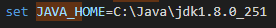
\includegraphics[scale=0.6]{img/part3/2.2}
    \caption{Site de téléchargement de Cassandra}
\end{figure}
\item Cliquez sur le lien de téléchargement miroir suggéré pour démarrer le processus de téléchargement.
\begin{figure}[h]
	\centering
    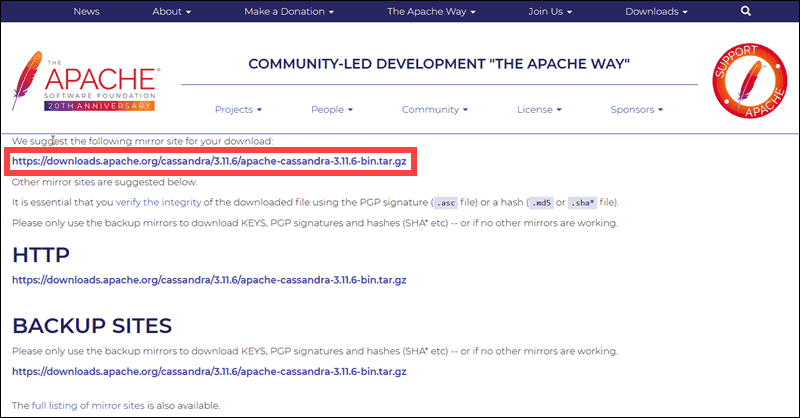
\includegraphics[scale=0.5]{img/part3/2.3}
    \caption{le lien de téléchargement miroir}
\end{figure}
\newpage
\item Décompressez le dossier tar.gz compressé à l'aide d'un outil de compression tel que 7-Zip ou WinZip. Dans cet exemple, le dossier compressé a été décompressé et le contenu placé dans le dossier C:/Cassandra/apache-cassandra-3.11.6.
\begin{figure}[h]
	\centering
    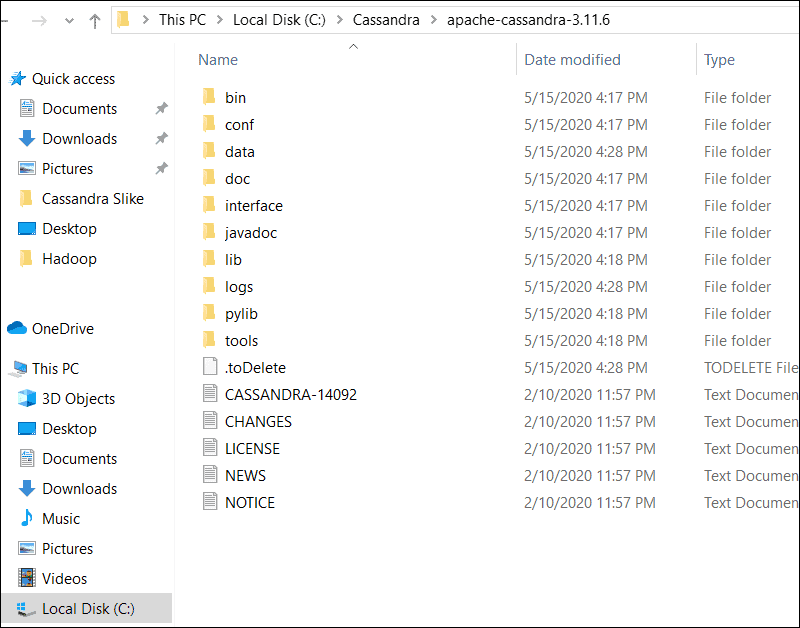
\includegraphics[scale=0.5]{img/part3/2.4}
    \caption{contenu du dossier}
\end{figure}
\end{enumerate}

\textbf{Configurer les variables d'environnement pour Cassandra:}

Configurez les variables d'environnement pour Cassandra afin de permettre à la base de données d'interagir avec d'autres applications et de fonctionner sous Windows.

\begin{enumerate}
\item Accédez à Ce PC > Propriétés.
\item Accédez à Paramètres système avancés .
\item Cliquez sur le bouton Variables d'environnement… .
\item Ajoutez une toute nouvelle entrée en sélectionnant l' option Nouveau .
\item Tapez $CASSANDRA_HOME$ pour Nom de la variable , puis pour la colonne Valeur de la variable , sélectionnez l'emplacement du  dossier Apache Cassandra décompressé.

Sur la base des étapes précédentes, l'emplacement est C:/Cassandra/apache-cassandra-3.11.6. Une fois que vous avez confirmé que l'emplacement est correct, cliquez sur OK.
\item Double-cliquez sur la variable Chemin .
\item Sélectionnez Nouveau puis Parcourir . Dans ce cas, vous devez ajouter le chemin complet du  dossier bin situé dans le dossier Apache Cassandra, C:/Cassandra/apache-cassandra-3.11.6bin .
\item Appuyez sur le bouton OK , puis à nouveau sur OK pour enregistrer les variables modifiées.
\end{enumerate}
\newpage
\subsubsection {Étape 3 : Démarrez Cassandra à partir de Windows CMD:}
Accédez au dossier Cassandra bin. Démarrez l'invite de commande Windows directement à partir du dossier bin en tapant cmd dans la barre d'adresse et en appuyant sur Entrée .

\begin{figure}[h]
	\centering
    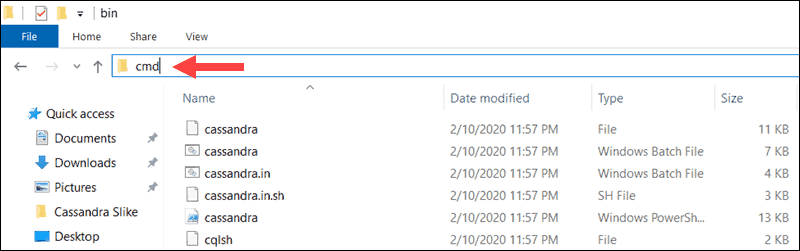
\includegraphics[scale=0.6]{img/part3/2.5}
    \caption{dossier Cassandra bin}
\end{figure}

Tapez la commande suivante pour démarrer le serveur Cassandra :

\begin{center}
$cassandra$
\end{center}

Le système démarre le serveur Cassandra.

\begin{figure}[h]
	\centering
    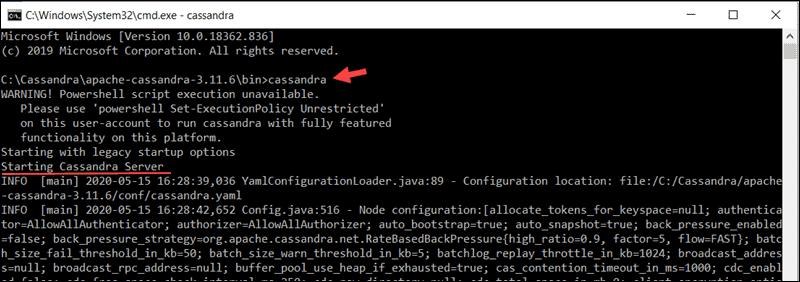
\includegraphics[scale=0.6]{img/part3/2.6}
    \caption{le serveur Cassandra}
\end{figure}

Ne fermez pas la session cmd en cours.
\newpage
\subsubsection {Étape 5 : Accédez à Cassandra cqlsh à partir de Windows CMD:}

Pendant que l'invite de commande initiale est toujours en cours d'exécution, ouvrez une nouvelle invite de ligne de commande à partir du même dossier bin. Saisissez la commande suivante pour accéder au shell bash Cassandra cqlsh :

\begin{center}
$cqlsh$
\end{center}
Vous avez maintenant accès au shell Cassandra et pouvez procéder à l'émission de commandes de base de données de base sur votre serveur Cassandra.

\begin{figure}[h]
	\centering
    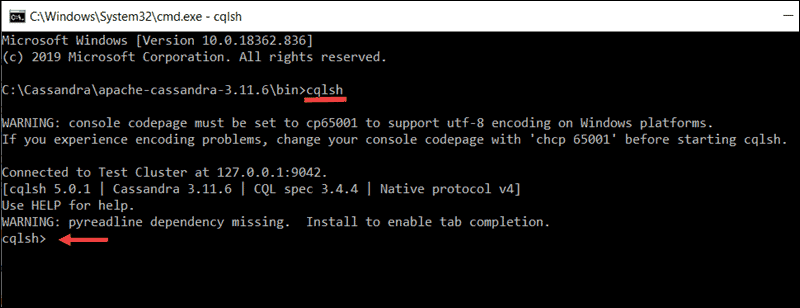
\includegraphics[scale=0.6]{img/part3/2.7}
    \caption{shell Cassandra}
\end{figure}